\documentclass{standalone}
\usepackage{pgfplots}
\pgfplotsset{compat=1.18}
\usepgfplotslibrary{fillbetween}

\begin{document}
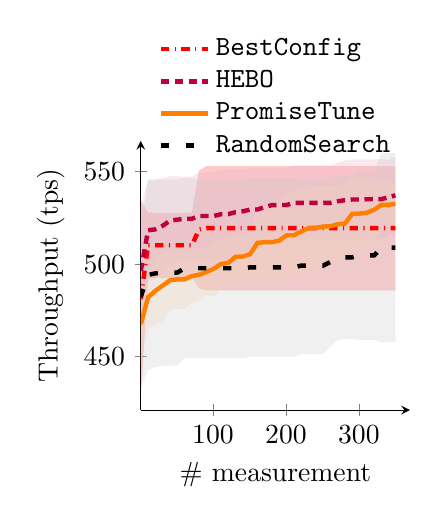
\begin{tikzpicture}
    \begin{axis}[
      axis x line  = bottom,
      axis y line  = left,
      width=5cm, height=5cm, 
      xlabel={\# measurement},
      ylabel={Throughput (tps)},
      xmin=1.0000, xmax=370.0000,
      ymin=421.2002, ymax=566.5312,
      legend cell align=left,
      legend columns=1,
      legend style={
        draw=none, fill=none,
        at={(0.98,0.9)}, anchor=south east,
        legend cell align=left
      }
    ]


\addplot[
    red,
    dashdotted,
    ultra thick, forget plot
] coordinates {
(1.0000, 481.0960) (11.0000, 510.1800) (21.0000, 510.1800) (31.0000, 510.1800) (41.0000, 510.1800) (51.0000, 510.1800) (61.0000, 510.1800) (71.0000, 510.1800) (81.0000, 518.7480) (91.0000, 519.4160) (101.0000, 519.4160) (111.0000, 519.4160) (121.0000, 519.4160) (131.0000, 519.4160) (141.0000, 519.4160) (151.0000, 519.4160) (161.0000, 519.4160) (171.0000, 519.4160) (181.0000, 519.4160) (191.0000, 519.4160) (201.0000, 519.4160) (211.0000, 519.4160) (221.0000, 519.4160) (231.0000, 519.4160) (241.0000, 519.4160) (251.0000, 519.4160) (261.0000, 519.4160) (271.0000, 519.4160) (281.0000, 519.4160) (291.0000, 519.4160) (301.0000, 519.4160) (311.0000, 519.4160) (321.0000, 519.4160) (331.0000, 519.4160) (341.0000, 519.4160) (350.0000, 519.4160)
}; 
\addlegendentry{\texttt{BestConfig}}

\addplot[
name path=upper0,
draw=none, forget plot
] coordinates {
(1.0000, 534.3859) (11.0000, 527.8734) (21.0000, 527.8734) (31.0000, 527.8734) (41.0000, 527.8734) (51.0000, 527.8734) (61.0000, 527.8734) (71.0000, 527.8734) (81.0000, 550.5998) (91.0000, 552.9533) (101.0000, 552.9533) (111.0000, 552.9533) (121.0000, 552.9533) (131.0000, 552.9533) (141.0000, 552.9533) (151.0000, 552.9533) (161.0000, 552.9533) (171.0000, 552.9533) (181.0000, 552.9533) (191.0000, 552.9533) (201.0000, 552.9533) (211.0000, 552.9533) (221.0000, 552.9533) (231.0000, 552.9533) (241.0000, 552.9533) (251.0000, 552.9533) (261.0000, 552.9533) (271.0000, 552.9533) (281.0000, 552.9533) (291.0000, 552.9533) (301.0000, 552.9533) (311.0000, 552.9533) (321.0000, 552.9533) (331.0000, 552.9533) (341.0000, 552.9533) (350.0000, 552.9533)
}; 

\addplot[
name path=lower0,
draw=none, forget plot
] coordinates {
(1.0000, 427.8061) (11.0000, 492.4866) (21.0000, 492.4866) (31.0000, 492.4866) (41.0000, 492.4866) (51.0000, 492.4866) (61.0000, 492.4866) (71.0000, 492.4866) (81.0000, 486.8962) (91.0000, 485.8787) (101.0000, 485.8787) (111.0000, 485.8787) (121.0000, 485.8787) (131.0000, 485.8787) (141.0000, 485.8787) (151.0000, 485.8787) (161.0000, 485.8787) (171.0000, 485.8787) (181.0000, 485.8787) (191.0000, 485.8787) (201.0000, 485.8787) (211.0000, 485.8787) (221.0000, 485.8787) (231.0000, 485.8787) (241.0000, 485.8787) (251.0000, 485.8787) (261.0000, 485.8787) (271.0000, 485.8787) (281.0000, 485.8787) (291.0000, 485.8787) (301.0000, 485.8787) (311.0000, 485.8787) (321.0000, 485.8787) (331.0000, 485.8787) (341.0000, 485.8787) (350.0000, 485.8787)
}; 

% ========= file shading =========
\addplot[
    red!70,
    fill opacity=0.30, forget plot
] fill between[
    of=upper0 and lower0,
];


\addplot[
    purple,
    densely dashed,
    ultra thick, forget plot
] coordinates {
(1.0000, 496.2700) (11.0000, 518.2660) (21.0000, 518.7800) (31.0000, 520.6880) (41.0000, 523.4530) (51.0000, 523.9870) (61.0000, 524.5030) (71.0000, 524.5030) (81.0000, 525.9930) (91.0000, 525.9930) (101.0000, 525.9930) (111.0000, 526.9650) (121.0000, 527.0110) (131.0000, 528.0680) (141.0000, 528.5000) (151.0000, 529.5010) (161.0000, 529.5010) (171.0000, 530.7940) (181.0000, 531.8700) (191.0000, 531.9410) (201.0000, 531.9410) (211.0000, 533.0500) (221.0000, 533.0500) (231.0000, 533.0500) (241.0000, 533.0500) (251.0000, 533.0500) (261.0000, 533.0990) (271.0000, 533.9280) (281.0000, 534.5360) (291.0000, 534.9080) (301.0000, 534.9080) (311.0000, 535.0260) (321.0000, 535.0640) (331.0000, 535.1380) (341.0000, 536.0540) (350.0000, 537.1710)
}; 
\addlegendentry{\texttt{HEBO}}

\addplot[
name path=upper1,
draw=none, forget plot
] coordinates {
(1.0000, 518.8411) (11.0000, 545.5214) (21.0000, 545.5614) (31.0000, 546.2547) (41.0000, 547.5455) (51.0000, 547.3332) (61.0000, 547.2123) (71.0000, 547.2123) (81.0000, 549.5526) (91.0000, 549.5526) (101.0000, 549.5526) (111.0000, 551.1223) (121.0000, 551.1142) (131.0000, 551.1225) (141.0000, 551.2395) (151.0000, 551.7849) (161.0000, 551.7849) (171.0000, 551.6136) (181.0000, 551.8933) (191.0000, 551.8389) (201.0000, 551.8389) (211.0000, 553.3608) (221.0000, 553.3608) (231.0000, 553.3608) (241.0000, 553.3608) (251.0000, 553.3608) (261.0000, 553.3233) (271.0000, 554.8233) (281.0000, 556.0932) (291.0000, 556.5757) (301.0000, 556.5757) (311.0000, 556.4986) (321.0000, 556.5862) (331.0000, 556.7581) (341.0000, 556.3125) (350.0000, 558.2336)
}; 

\addplot[
name path=lower1,
draw=none, forget plot
] coordinates {
(1.0000, 473.6989) (11.0000, 491.0106) (21.0000, 491.9986) (31.0000, 495.1213) (41.0000, 499.3605) (51.0000, 500.6408) (61.0000, 501.7937) (71.0000, 501.7937) (81.0000, 502.4334) (91.0000, 502.4334) (101.0000, 502.4334) (111.0000, 502.8077) (121.0000, 502.9078) (131.0000, 505.0135) (141.0000, 505.7605) (151.0000, 507.2171) (161.0000, 507.2171) (171.0000, 509.9744) (181.0000, 511.8467) (191.0000, 512.0431) (201.0000, 512.0431) (211.0000, 512.7392) (221.0000, 512.7392) (231.0000, 512.7392) (241.0000, 512.7392) (251.0000, 512.7392) (261.0000, 512.8747) (271.0000, 513.0327) (281.0000, 512.9788) (291.0000, 513.2403) (301.0000, 513.2403) (311.0000, 513.5534) (321.0000, 513.5418) (331.0000, 513.5179) (341.0000, 515.7955) (350.0000, 516.1084)
}; 

% ========= file shading =========
\addplot[
    purple!30,
    fill opacity=0.30, forget plot
] fill between[
    of=upper1 and lower1,
];


\addplot[
    orange,
    solid,
    ultra thick, forget plot
] coordinates {
(1.0000, 467.5960) (11.0000, 482.0850) (21.0000, 485.5710) (31.0000, 488.4250) (41.0000, 491.2260) (51.0000, 491.8130) (61.0000, 491.8130) (71.0000, 493.5130) (81.0000, 494.2840) (91.0000, 495.7390) (101.0000, 497.4820) (111.0000, 500.1000) (121.0000, 500.6750) (131.0000, 503.9730) (141.0000, 504.0950) (151.0000, 505.4510) (161.0000, 511.4950) (171.0000, 511.8550) (181.0000, 511.8550) (191.0000, 512.7290) (201.0000, 515.5860) (211.0000, 515.5860) (221.0000, 517.5920) (231.0000, 519.4780) (241.0000, 519.5590) (251.0000, 520.3180) (261.0000, 520.4130) (271.0000, 521.5390) (281.0000, 521.9200) (291.0000, 527.1940) (301.0000, 527.2740) (311.0000, 527.7650) (321.0000, 529.3730) (331.0000, 532.0360) (341.0000, 532.0360) (350.0000, 532.6020)
}; 
\addlegendentry{\texttt{PromiseTune}}

\addplot[
name path=upper2,
draw=none, forget plot
] coordinates {
(1.0000, 488.0951) (11.0000, 498.9967) (21.0000, 504.1404) (31.0000, 507.4529) (41.0000, 506.9238) (51.0000, 507.7374) (61.0000, 507.7374) (71.0000, 507.9805) (81.0000, 508.2784) (91.0000, 508.2354) (101.0000, 512.3593) (111.0000, 513.5613) (121.0000, 513.7702) (131.0000, 515.9685) (141.0000, 516.0026) (151.0000, 516.7143) (161.0000, 530.1905) (171.0000, 530.4104) (181.0000, 530.4104) (191.0000, 532.5001) (201.0000, 538.6195) (211.0000, 538.6195) (221.0000, 539.9045) (231.0000, 542.0796) (241.0000, 542.0549) (251.0000, 542.0986) (261.0000, 542.0911) (271.0000, 542.1913) (281.0000, 542.5777) (291.0000, 546.3183) (301.0000, 546.4251) (311.0000, 546.6664) (321.0000, 546.5122) (331.0000, 545.4521) (341.0000, 545.4521) (350.0000, 546.2087)
}; 

\addplot[
name path=lower2,
draw=none, forget plot
] coordinates {
(1.0000, 447.0969) (11.0000, 465.1733) (21.0000, 467.0016) (31.0000, 469.3971) (41.0000, 475.5282) (51.0000, 475.8886) (61.0000, 475.8886) (71.0000, 479.0455) (81.0000, 480.2896) (91.0000, 483.2426) (101.0000, 482.6047) (111.0000, 486.6387) (121.0000, 487.5798) (131.0000, 491.9775) (141.0000, 492.1874) (151.0000, 494.1877) (161.0000, 492.7995) (171.0000, 493.2996) (181.0000, 493.2996) (191.0000, 492.9579) (201.0000, 492.5525) (211.0000, 492.5525) (221.0000, 495.2795) (231.0000, 496.8764) (241.0000, 497.0631) (251.0000, 498.5374) (261.0000, 498.7349) (271.0000, 500.8867) (281.0000, 501.2623) (291.0000, 508.0697) (301.0000, 508.1229) (311.0000, 508.8636) (321.0000, 512.2338) (331.0000, 518.6199) (341.0000, 518.6199) (350.0000, 518.9953)
}; 

% ========= file shading =========
\addplot[
    orange!30,
    fill opacity=0.30, forget plot
] fill between[
    of=upper2 and lower2,
];


\addplot[
    black,
    loosely dashed,
    ultra thick, forget plot
] coordinates {
(1.0000, 482.2910) (11.0000, 494.2030) (21.0000, 495.0030) (31.0000, 495.4000) (41.0000, 495.4000) (51.0000, 495.4000) (61.0000, 497.7790) (71.0000, 497.7790) (81.0000, 497.7790) (91.0000, 497.7790) (101.0000, 497.7790) (111.0000, 497.7790) (121.0000, 497.7790) (131.0000, 497.7790) (141.0000, 497.7790) (151.0000, 498.2570) (161.0000, 498.2570) (171.0000, 498.2570) (181.0000, 498.2570) (191.0000, 498.2570) (201.0000, 498.2570) (211.0000, 498.2570) (221.0000, 499.2090) (231.0000, 499.2090) (241.0000, 499.2090) (251.0000, 499.2090) (261.0000, 501.1610) (271.0000, 503.3320) (281.0000, 503.6860) (291.0000, 503.6860) (301.0000, 504.7540) (311.0000, 504.7540) (321.0000, 504.7540) (331.0000, 508.9000) (341.0000, 508.9000) (350.0000, 508.9000)
}; 
\addlegendentry{\texttt{RandomSearch}}

\addplot[
name path=upper3,
draw=none, forget plot
] coordinates {
(1.0000, 531.5108) (11.0000, 545.5820) (21.0000, 545.5936) (31.0000, 545.6374) (41.0000, 545.6374) (51.0000, 545.6374) (61.0000, 546.3325) (71.0000, 546.3325) (81.0000, 546.3325) (91.0000, 546.3325) (101.0000, 546.3325) (111.0000, 546.3325) (121.0000, 546.3325) (131.0000, 546.3325) (141.0000, 546.3325) (151.0000, 546.4948) (161.0000, 546.4948) (171.0000, 546.4948) (181.0000, 546.4948) (191.0000, 546.4948) (201.0000, 546.4948) (211.0000, 546.4948) (221.0000, 546.8322) (231.0000, 546.8322) (241.0000, 546.8322) (251.0000, 546.8322) (261.0000, 546.6610) (271.0000, 547.7233) (281.0000, 547.7831) (291.0000, 547.7831) (301.0000, 550.5813) (311.0000, 550.5813) (321.0000, 550.5813) (331.0000, 559.9252) (341.0000, 559.9252) (350.0000, 559.9252)
}; 

\addplot[
name path=lower3,
draw=none, forget plot
] coordinates {
(1.0000, 433.0712) (11.0000, 442.8240) (21.0000, 444.4124) (31.0000, 445.1626) (41.0000, 445.1626) (51.0000, 445.1626) (61.0000, 449.2255) (71.0000, 449.2255) (81.0000, 449.2255) (91.0000, 449.2255) (101.0000, 449.2255) (111.0000, 449.2255) (121.0000, 449.2255) (131.0000, 449.2255) (141.0000, 449.2255) (151.0000, 450.0192) (161.0000, 450.0192) (171.0000, 450.0192) (181.0000, 450.0192) (191.0000, 450.0192) (201.0000, 450.0192) (211.0000, 450.0192) (221.0000, 451.5858) (231.0000, 451.5858) (241.0000, 451.5858) (251.0000, 451.5858) (261.0000, 455.6610) (271.0000, 458.9407) (281.0000, 459.5889) (291.0000, 459.5889) (301.0000, 458.9267) (311.0000, 458.9267) (321.0000, 458.9267) (331.0000, 457.8748) (341.0000, 457.8748) (350.0000, 457.8748)
}; 

% ========= file shading =========
\addplot[
    black!20,
    fill opacity=0.30, forget plot
] fill between[
    of=upper3 and lower3,
];


\addlegendimage{red, dashdotted, ultra thick}
\addlegendentry{\texttt{BestConfig}}
\addlegendimage{purple, densely dashed, ultra thick}
\addlegendentry{\texttt{HEBO}}
\addlegendimage{orange, solid, ultra thick}
\addlegendentry{\texttt{PromiseTune}}
\addlegendimage{black, loosely dashed, ultra thick}
\addlegendentry{\texttt{RandomSearch}}

\end{axis}
\end{tikzpicture}
\end{document}
